\documentclass[11pt]{article}

\usepackage[margin=1in]{geometry}
\usepackage{amsmath,amssymb,amsthm}
\usepackage{mathpazo}
\usepackage{microtype}
\usepackage{graphicx}
\usepackage{booktabs}
\usepackage{tabularx}
\usepackage[dvipsnames]{xcolor}
\usepackage{enumitem}
\usepackage{fancyhdr}
\usepackage[most]{tcolorbox}
\usepackage[round,authoryear]{natbib}
\usepackage[colorlinks=true,linkcolor=NavyBlue,citecolor=NavyBlue,urlcolor=NavyBlue]{hyperref}

\definecolor{navy}{HTML}{1F3A5F}
\newtheorem{proposition}{Proposition}
\newtheorem{lemma}{Lemma}
\theoremstyle{definition}
\newtheorem{definition}{Definition}
\newtheorem{remark}{Remark}

\newcommand{\E}{\mathbb{E}}
\newcommand{\Var}{\operatorname{Var}}
\newcommand{\sgn}{\operatorname{sgn}}
\newcommand{\1}{\mathbf{1}}
\newcommand{\F}{\mathcal{F}}

\pagestyle{fancy}
\fancyhf{}
\lhead{\small\textsc{PEAD: Underreaction, Convexity, and Growth-Optimal Sizing}}
\rhead{\small\thepage}
\renewcommand{\headrulewidth}{0.4pt}

\setlist{itemsep=2pt,topsep=4pt}

\title{\vspace{-1.2cm}\textbf{Underreaction, Convexity, and Growth-Optimal Sizing:\\[2pt]
Harvesting Post-Earnings-Announcement Drift\\ in the Equity and Options Markets}}
\author{Hrudith L.\\[2pt] \small PEAD Trading Research}
\date{September 2026}

\begin{document}
\maketitle
\thispagestyle{empty}

\begin{abstract}
\noindent
We document, model, and trade post-earnings-announcement drift (PEAD) in two markets
at once. On 182{,}712 analyst-based earnings surprises (1996--2013) the top-minus-bottom
surprise-decile spread is $+3.05\%$ over 60 trading days ($t=5.25$, clustered by
announcement quarter). It rises to $+3.76\%$ ($t=9.25$) after a leave-one-out size and
book-to-market adjustment, so the drift is not a size or value premium in disguise. The
same ordering shows up in listed options: near-the-money calls on the most positive
surprises beat those on the most negative by $+14.38\%$ of premium ($t=4.69$), and puts
show the mirror image ($-10.79\%$, $t=-6.29$). We turn the signal into two books. The first
is a sector- and size-neutral, market-hedged equity long/short book. Its holding periods
come from an empirical, cell-level decay-time estimator, and it is scaled to its
capacity-constrained optimum. It returns $12.15\%$ a year at $12.20\%$ volatility (Sharpe
$1.00$), with a market beta of $-0.015$. The second is a long-only options book. For every
event it scans the full option chain and picks the contract that maximizes expected
logarithmic growth $\E[\log(1+fR)]$ under a walk-forward, decile-conditioned empirical
distribution. It then spreads a fixed premium budget across concurrent bets in proportion
to their Kelly fractions. At a 30\% outstanding-premium budget it returns $12.26\%$ a year at
$3.33\%$ volatility (Sharpe $3.49$), and every position's loss is capped at its premium. The
two books have a daily return correlation of $-0.05$. We derive the relevant properties of the
selector: its second-order equivalence to Sharpe-ratio ranking, the minimum-stake hurdle
that removes lottery-ticket strikes, and the fact that proportional budget allocation is
fractional Kelly with an endogenous fraction near $2\times10^{-3}$. We also derive a capacity
bound for the equity book, and we report deflated Sharpe ratios, a full log of the backtest
defects we found and fixed, and the limitations that matter for deployment.
\end{abstract}

\begin{tcolorbox}[colback=navy!4,colframe=navy,title=\textbf{Key results (backtest, 1996--2013, \$10M initial capital, net of modeled costs)},fonttitle=\small,left=4pt,right=4pt,top=3pt,bottom=3pt]
\small
\begin{tabularx}{\linewidth}{@{}Xrrrrr@{}}
\toprule
Book & Ann.\ ret. & Ann.\ vol & Sharpe & Max DD & Corr.\ to mkt \\
\midrule
Equity long/short (sector/size-neutral) & 12.15\% & 12.20\% & 1.00 & $-36.5\%$ & $-0.02$ \\
Kelly options (60d, $c=30\%$) & 12.26\% & 3.33\% & 3.49 & $-17.4\%$ & $0.20$ \\
50/50 blend, 1998--2013$^\dagger$ & 12.73\% & 6.48\% & 1.88 & $-18.5\%$ & -- \\
\bottomrule
\end{tabularx}
\vspace{2pt}
{\footnotesize $^\dagger$Illustrative blend computed from the two books' daily NAV series; not a separately backtested strategy.
All figures are hypothetical backtest results; see Section~\ref{sec:limits}.}
\end{tcolorbox}

\tableofcontents
\newpage

%=====================================================================================
\section{Introduction}
%=====================================================================================

Post-earnings-announcement drift is one of the oldest and most persistent anomalies in
empirical finance. After a firm reports earnings that differ from expectations, its price
does not adjust fully on the announcement. Over the following weeks it keeps moving in the
direction of the surprise \citep{BallBrown1968,BernardThomas1989,BernardThomas1990}. The
leading explanations are behavioral underreaction and investor inattention
\citep{HirshleiferLimTeoh2009,DellaVignaPollet2009}, together with limits to arbitrage that
keep informed capital from closing the gap quickly
\citep{ShleiferVishny1997,Mendenhall2004}.

For a practitioner, the drift raises three distinct engineering problems, and this paper
takes them in order.
\begin{enumerate}[label=(\roman*)]
  \item \textbf{Identification.} Is the drift in this data a real mispricing, statistically
        robust to the heavy cross-sectional dependence of earnings seasons? Or is it
        compensation for size and value exposure? And does it persist in a second,
        independently priced market (listed options)?
  \item \textbf{Linear harvesting.} Given a noisy, decaying, size-dependent cross-sectional
        signal, what portfolio isolates it? What holding period does the data support, and
        where does capacity bind?
  \item \textbf{Convex harvesting.} Options give leverage and bounded loss, but a naive
        expected-value contract selector is attracted to low-probability, high-payoff strikes.
        What selection and sizing rule turns a directional edge in the underlying into
        compounding capital growth?
\end{enumerate}

\paragraph{Contributions.}
(1) A quarter-clustered event study, a characteristic-adjusted robustness test, and
heterogeneity tests establish PEAD in an OptionMetrics-linked universe of 6{,}766
firms. The same design, applied to option premia, shows the signal carries into options
with an amplification of about $4.7\times$, in line with option elasticity.
(2) An equity construction that is dollar-, sector- and size-neutral, with holding periods
set by a nonparametric decay-time estimator for each (decile $\times$ size $\times$
book-to-market) cell. We characterize its capacity frontier analytically and empirically.
(3) A growth-optimal options selector. It scores every strike in the day-0 chain against a
walk-forward empirical return law, and we prove the properties that make it robust to
convexity traps.
(4) A joint view: the two books are almost uncorrelated, and in the one regime where the
linear book suffers most (the 2009 junk rally), the convex book gains.

\paragraph{Scope.} Across the project, eight equity constructions and several options
variants were built. This paper treats only the two final designs as ``the strategy'': the
highest-return equity construction, which runs at about 12\%, and the Kelly-optimal options
book. Earlier variants appear only where they explain a design choice.

%=====================================================================================
\section{Data and sample construction}\label{sec:data}
%=====================================================================================

\paragraph{Sources.} I/B/E/S analyst consensus and actuals; CRSP daily returns and the CRSP
value-weighted index $r_{m,t}$ (\texttt{vwretd}); Compustat annual common equity
(\texttt{ceq}); OptionMetrics IvyDB daily option quotes (about $7.5\times10^8$ option-day
records). The equity universe is every CRSP common stock that had listed options at some
point in the window: 8{,}115 PERMNOs.

\paragraph{Events.} An event $i$ is a firm-quarter earnings announcement with a resolved
day-0 session (the first trading day at or after the announcement). The surprise is
analyst-based. The consensus is restricted to snapshots dated strictly before the
announcement (\texttt{statpers} $<$ \texttt{anndats}), and both actual and forecast are
corrected for splits between consensus and announcement. We write
\begin{equation}
  \mathrm{SUE}_i \;=\; \frac{A_i - F_i}{s_i},
\end{equation}
where $A_i$ is realized EPS, $F_i$ the latest point-in-time consensus, and $s_i>0$ the
firm-specific scale used by the upstream pipeline. Analyst-sourced and seasonal
(time-series) surprises sit on different scales (sample s.d.\ 9.01 vs.\ 3.36), so they are
not pooled. The final sample is 182{,}712 events on 6{,}766 firms across $Q=72$ announcement
quarters (Table~\ref{tab:sample}).

\begin{table}[h]\centering\small
\caption{Sample construction.}\label{tab:sample}
\begin{tabular}{lr}
\toprule
Candidate earnings events, 1996--2013 & 268{,}606 \\
\quad with resolved day-0 session & 261{,}537 \\
\quad with analyst-based surprise (headline sample) & 182{,}712 \\
\quad with point-in-time book equity and size (characteristic-adjusted sample) & 175{,}016 \\
Linkable to an OptionMetrics \texttt{secid} (1:1 links only) & 164{,}673 \\
\quad matched to a near-ATM call or put with $\geq 95$ DTE on day 0 & 126{,}008 \\
\quad priced by the walk-forward Kelly selector (after 8-quarter warm-up) & 113{,}927 \\
\bottomrule
\end{tabular}
\end{table}

\paragraph{Returns.} For event $i$ with day-0 index $t_0$, the market-adjusted cumulative
return to horizon $h$ is
$\mathrm{CAR}_i(h)=\prod_{k=1}^{h}(1+r_{i,t_0+k})-\prod_{k=1}^{h}(1+r_{m,t_0+k})$, with
$h\in\{1,5,10,20,40,60\}$ trading days. Accrual starts on day $t_0+1$, so the
announcement-day reaction is not counted as drift. This matters for the leakage discussion
in Section~\ref{sec:audit}.

%=====================================================================================
\section{Establishing the anomaly}\label{sec:evidence}
%=====================================================================================

\subsection{Point-in-time decile assignment}

Let $\mathcal{I}_q$ be the events announced in calendar quarter $q$. Each event gets its
within-quarter percentile rank
\begin{equation}
  u_i = \frac{1}{|\mathcal{I}_q|}\,\mathrm{rank}_{\,j\in\mathcal{I}_q}\!\big(\mathrm{SUE}_j\big)\in(0,1],
  \qquad D_i=\min\big(\lceil 10\,u_i\rceil,10\big),
\end{equation}
with average ranks for ties (SUE rounded to $10^{-8}$). Ranking inside the quarter keeps
the breakpoints free of multi-year look-ahead. The residual intra-quarter look-ahead is
discussed in Section~\ref{sec:limits}. 11.6\% of surprises are exactly zero, so $D_4$ holds
22{,}423 events against about 15{,}000--19{,}000 in the other deciles. That imbalance is a
property of the data, not a defect of the sort.

\subsection{Inference under earnings-season clustering}

Announcements cluster heavily inside each reporting season, and returns of firms
announcing in the same season share common shocks. An i.i.d.\ standard error over 182{,}712
events would badly overstate precision. We use the Fama--MacBeth estimator
\citep{FamaMacBeth1973}, taking the announcement quarter as the unit of observation. For any
event-level quantity $x_i$ and event set $\mathcal{S}$,
\begin{equation}
  \bar x_q=\frac{1}{|\mathcal{S}\cap\mathcal{I}_q|}\sum_{i\in\mathcal{S}\cap\mathcal{I}_q}x_i,\qquad
  \hat\mu=\frac1Q\sum_{q=1}^{Q}\bar x_q,\qquad
  \widehat{\mathrm{SE}}(\hat\mu)=\frac{1}{\sqrt Q}\Big[\tfrac{1}{Q-1}\textstyle\sum_q(\bar x_q-\hat\mu)^2\Big]^{1/2}.
  \label{eq:fm}
\end{equation}
This estimator is consistent under arbitrary within-quarter dependence. The long/short
spread is formed \emph{at the quarter level},
$\Delta_q(h)=\overline{\mathrm{CAR}}_{q,D10}(h)-\overline{\mathrm{CAR}}_{q,D1}(h)$, so its
standard error reflects the fact that both legs are drawn from the same cross-section.

\subsection{Headline result}

\begin{figure}[t]\centering
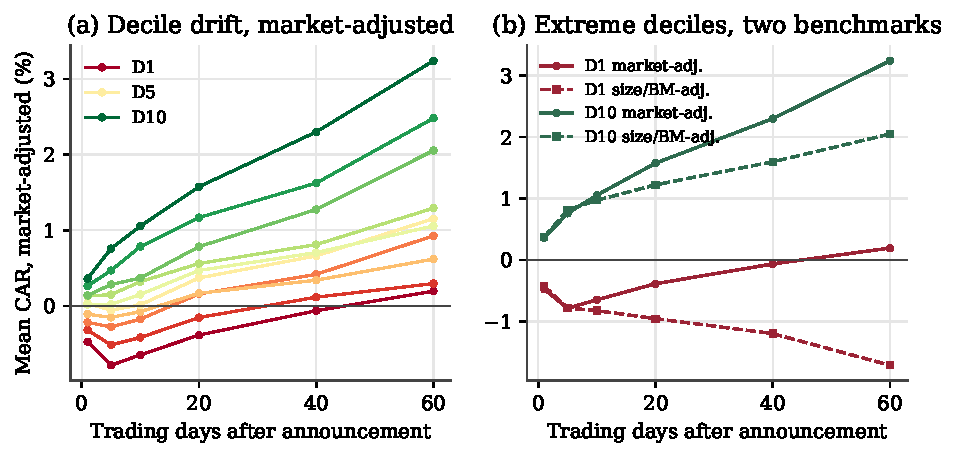
\includegraphics[width=\linewidth]{figures/fig1_decile_drift.pdf}
\caption{(a) Mean market-adjusted CAR by SUE decile. The ordering is monotone from $+10$
days onward. (b) Extreme deciles under the market benchmark (solid) and under the
leave-one-out size/book-to-market benchmark (dashed). Once size and value are controlled
for, D1 declines monotonically to $-1.71\%$.}\label{fig:drift}
\end{figure}

\begin{table}[t]\centering\small
\caption{Mean market-adjusted CAR (\%) by SUE decile and horizon; Fama--MacBeth means over 72 quarters.}\label{tab:deciles}
\begin{tabular}{lrrrrrr}
\toprule
Decile & $+1$d & $+5$d & $+10$d & $+20$d & $+40$d & $+60$d \\
\midrule
D1 (most negative) & $-0.47$ & $-0.79$ & $-0.65$ & $-0.39$ & $-0.06$ & $+0.19$ \\
D2 & $-0.32$ & $-0.52$ & $-0.42$ & $-0.15$ & $+0.11$ & $+0.29$ \\
D3 & $-0.22$ & $-0.28$ & $-0.18$ & $+0.16$ & $+0.42$ & $+0.93$ \\
D4 & $-0.11$ & $-0.15$ & $-0.08$ & $+0.17$ & $+0.34$ & $+0.62$ \\
D5 & $+0.03$ & $-0.06$ & $+0.01$ & $+0.37$ & $+0.66$ & $+1.15$ \\
D6 & $+0.02$ & $+0.02$ & $+0.15$ & $+0.47$ & $+0.70$ & $+1.06$ \\
D7 & $+0.13$ & $+0.15$ & $+0.32$ & $+0.56$ & $+0.81$ & $+1.29$ \\
D8 & $+0.14$ & $+0.28$ & $+0.37$ & $+0.78$ & $+1.27$ & $+2.05$ \\
D9 & $+0.26$ & $+0.47$ & $+0.78$ & $+1.17$ & $+1.62$ & $+2.48$ \\
D10 (most positive) & $+0.36$ & $+0.76$ & $+1.05$ & $+1.57$ & $+2.30$ & $+3.24$ \\
\bottomrule
\end{tabular}
\end{table}

\begin{table}[t]\centering\small
\caption{D10 $-$ D1 spread by horizon, with quarter-clustered $t$-statistics. Equity columns
use the full event sample; option columns use the option-matched subsample (67 quarters;
65 at $+60$d) and measure the return on premium of a buy-and-hold near-ATM contract at
mid.}\label{tab:spreads}
\begin{tabular}{l rr rr rr rr rr}
\toprule
 & \multicolumn{2}{c}{Mkt-adj.\ equity} & \multicolumn{2}{c}{Size/BM-adj.\ equity} & \multicolumn{2}{c}{Call} & \multicolumn{2}{c}{Put} & \multicolumn{2}{c}{Straddle}\\
\cmidrule(lr){2-3}\cmidrule(lr){4-5}\cmidrule(lr){6-7}\cmidrule(lr){8-9}\cmidrule(lr){10-11}
Horizon & $\hat\mu$ & $t$ & $\hat\mu$ & $t$ & $\hat\mu$ & $t$ & $\hat\mu$ & $t$ & $\hat\mu$ & $t$\\
\midrule
$+1$d  & 0.83 & 10.90 & 0.80 & 11.41 & 4.01 & 13.33 & $-2.49$ & $-13.21$ & 0.27 & 3.31\\
$+5$d  & 1.54 & 12.23 & 1.59 & 14.21 & 8.03 & 13.27 & $-5.11$ & $-13.04$ & 0.77 & 4.61\\
$+10$d & 1.70 & 10.17 & 1.79 & 12.30 & 9.54 & 11.87 & $-5.86$ & $-13.01$ & 1.24 & 4.87\\
$+20$d & 1.96 & 8.74  & 2.18 & 12.09 & 11.29 & 8.34 & $-6.46$ & $-7.91$ & 2.18 & 4.97\\
$+40$d & 2.36 & 5.64  & 2.79 & 9.68  & 11.76 & 5.67 & $-8.27$ & $-6.64$ & 2.80 & 5.10\\
$+60$d & 3.05 & 5.25  & 3.76 & 9.25  & 14.38 & 4.69 & $-10.79$ & $-6.29$ & 3.98 & 5.22\\
\bottomrule
\end{tabular}
\end{table}

Table~\ref{tab:deciles} and Figure~\ref{fig:drift} show the canonical PEAD pattern. The
decile means are ordered at every horizon, and from $+10$ days the ordering is strictly
monotone. The spread grows with horizon, from $0.83\%$ at one day to $3.05\%$ at 60 days
(Table~\ref{tab:spreads}), and every clustered $t$-statistic exceeds $5.2$. A spread that
keeps growing is what gradual incorporation of information predicts. A one-off reaction
that merely differs by decile would produce a flat spread.

\subsection{Risk-based explanations: a leave-one-out characteristic benchmark}

In market-adjusted terms, D1 recovers after day 20. One reading is that extreme-bad-news
firms are small, high book-to-market firms that earn a size/value premium, which would
make part of the ``drift'' risk compensation. We test this with a characteristic
benchmark in the spirit of \citet{DGTW1997}. Each event is assigned to a cell
$c(i)=(q,\ \text{size quintile},\ \text{BM tercile})$. Book equity comes from Compustat
\texttt{ceq}$>0$ with at least a 130-day reporting lag, both sorts are formed within the
quarter, and 175{,}016 events are covered. The adjusted return is
\begin{equation}
  \widetilde{\mathrm{CAR}}_i(h)=\mathrm{CAR}_i(h)-\frac{\sum_{j\in c(i)}\mathrm{CAR}_j(h)-\mathrm{CAR}_i(h)}{n_{c(i)}-1}.
  \label{eq:loo}
\end{equation}
Leaving the event out stops its own return from shrinking its abnormal return toward zero,
an effect that matters in thin cells. After adjustment the spread is \emph{larger} at every
horizon ($3.76\%$ at 60d, $t=9.25$), and D1 no longer recovers
(Figure~\ref{fig:drift}b). What looked like a D1 reversal was a size/value premium sitting
on top of the drift. Adjusting for characteristics removes that premium and exposes the
drift in full.

\subsection{Heterogeneity and pooling}

\begin{figure}[t]\centering
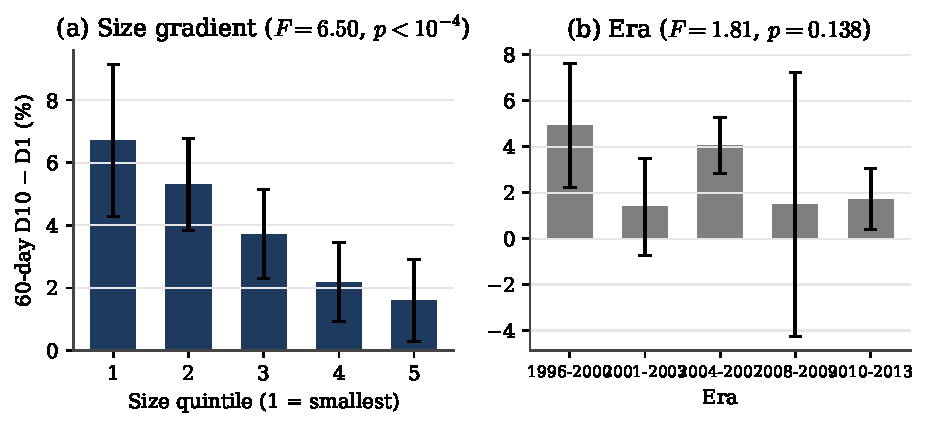
\includegraphics[width=\linewidth]{figures/fig3_heterogeneity.pdf}
\caption{60-day D10$-$D1 spread with 95\% confidence intervals by (a) size quintile at
announcement and (b) era. One-way ANOVA across the groups' quarterly spread series.}\label{fig:het}
\end{figure}

For grouping variable $g$ we compute the 60-day quarterly spread series
$\{\Delta^{(g)}_q\}$ separately within each group and test equality of means with a
one-way ANOVA.
\begin{itemize}
  \item \textbf{Sector (FF12):} $F=0.30$, $p=0.986$. Point estimates run from $0.98\%$
        (Chemicals) to $3.84\%$ (Finance), and every confidence interval overlaps every
        other. One pooled model across sectors is statistically justified.
  \item \textbf{Size:} $F=6.50$, $p<10^{-4}$. The spread falls monotonically from $6.71\%$
        ($t=5.43$) in the smallest quintile to $1.60\%$ ($t=2.41$) in the largest
        (Figure~\ref{fig:het}a). This is the limits-to-arbitrage signature: the drift is
        biggest where arbitrage is most expensive. Size therefore must be neutralized in
        construction and cannot simply be pooled.
  \item \textbf{Era:} $F=1.81$, $p=0.138$. Point estimates fall from $4.92\%$ (1996--2000)
        to $1.4$--$1.7\%$ after 2008, consistent with post-publication decay
        \citep{McLeanPontiff2016}. The decline is suggestive but not statistically
        significant.
\end{itemize}

\subsection{Rival hypotheses that were tested and rejected}

\paragraph{Surprise reversal.} \citet{BernardThomas1990} report a lag-4 SUE
autocorrelation of about $-0.24$. On 141{,}406 firm pairs we estimate $+0.05$. Firms in
the top decile four quarters earlier still average $\mathrm{SUE}_t=1.44$, against $-0.58$
for the bottom decile. The data show persistence, not reversal, so neither book fades a
firm's own past surprise.

\paragraph{Announcement-return (EAR) augmentation.} Blending the day-0 return into the
signal leaves the Sharpe ratio flat between 1.00 and 1.06 across blend weights. That holds
once EAR is restricted to information realized \emph{before} the first accrual day. An
earlier specification used the day-0-to-day-1 return, which overlaps a position's first day
of P\&L, and it produced a spurious Sharpe that kept rising with the blend weight. That
leak is logged in Section~\ref{sec:audit}.

\subsection{Cross-market confirmation: the options market}

If PEAD is a real mispricing of the underlying, it should also appear, amplified, in the
premium of a leveraged claim on that underlying. For each option-linked event we pick, on
day 0, the call (put) with $\Delta$ closest to $+0.5$ ($-0.5$). The contract needs a
two-sided quote and at least 95 calendar days to expiry, and ties are broken toward 120 DTE.
We hold it at mid, with no rolling, to each horizon. The inference is the estimator in
\eqref{eq:fm}.

\paragraph{Magnitude.} For a call with price $C$ and delta $\Delta$, the Black--Scholes
elasticity is $\Omega=\Delta S/C$. At the money $C\approx 0.4\,S\sigma\sqrt T$, so
$\Omega\approx\Delta/(0.4\,\sigma\sqrt T)$. With $\Delta\approx 0.5$, $T\approx 1/3$ and
$\sigma\in[0.35,0.45]$, $\Omega\approx 4.8$--$6.2$. The observed ratio of the 60-day call
spread to the stock spread is $14.38/3.05\approx 4.7$. That sits just below the elasticity
band, as expected once theta and vega act on a position held for 60 days. So the options
market carries the same directional signal, scaled by leverage (Table~\ref{tab:spreads},
Figure~\ref{fig:spreads}b).

\paragraph{Direction versus volatility.} A long straddle has close to zero delta and so
isolates the non-directional component. Its 60-day spread is $+3.98\%$ ($t=5.22$), about a
quarter of the call spread. Extreme-surprise names therefore carry a secondary
volatility component. That component is small next to the directional one, which remains
the primary effect.

\begin{figure}[t]\centering
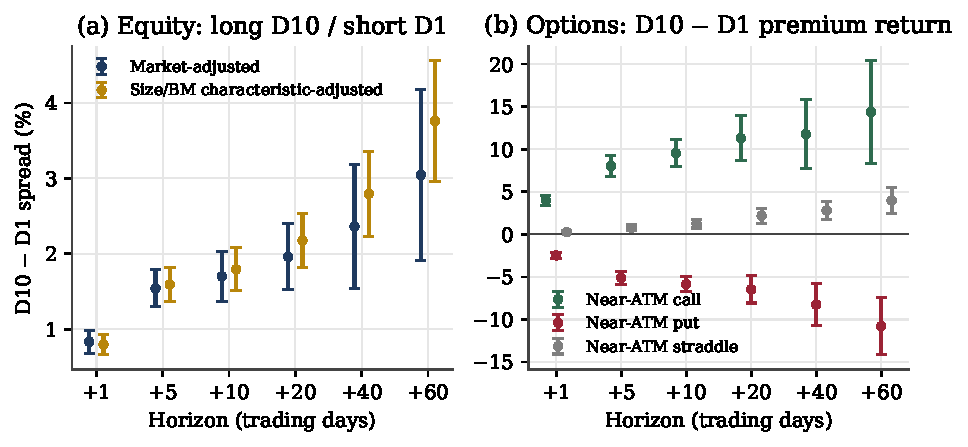
\includegraphics[width=\linewidth]{figures/fig2_spreads.pdf}
\caption{D10$-$D1 spreads with 95\% quarter-clustered confidence intervals. (a) Equity,
market-adjusted and characteristic-adjusted. (b) Near-ATM options, as return on premium.}\label{fig:spreads}
\end{figure}

\subsection{Decay kinetics and the holding-period estimator}\label{sec:decay}

A trading rule has to decide when the marginal day of holding stops paying. Let
$\overline{\mathrm{CAR}}_c(d)$ be the Fama--MacBeth mean characteristic-adjusted CAR of
holding cell $c$ on day $d=1,\dots,200$. The cells are decile $\times$ size $\times$
book-to-market. A cell with fewer than 20 quarters or 400 events backs off to decile
$\times$ size, and then to decile alone; 138 fine and 6 medium cells survive. Daily marginal
returns are too noisy to threshold directly, so we use a trailing windowed slope and a
cell-specific relative threshold:
\begin{align}
  \varsigma_c(d)&=\tfrac{1}{W}\big[\overline{\mathrm{CAR}}_c(d)-\overline{\mathrm{CAR}}_c(d-W)\big],\qquad W=20,\\
  \theta_c&=0.15\max_{d\le 90}|\varsigma_c(d)|,\\
  \mathcal{E}_c(d)&=\big\{|\varsigma_c(d)|<\theta_c\big\}\ \cup\ \big\{\sgn\varsigma_c(d)\neq s_c\big\},\\
  H_c&=\min\Big\{d\ge 30:\ \textstyle\bigcap_{k=d}^{d+9}\mathcal{E}_c(k)\Big\},
\end{align}
where $s_c=+1$ for deciles $6$--$10$ and $-1$ otherwise. In words, $H_c$ is the first day
after a 30-day burn-in on which the drift rate has fallen below 15\% of its own peak, or
turned the wrong way, and stays there for ten consecutive days. Across cells $H_c$ ranges
from 31 to 200 trading days (median 49, mean 57). It is longest in the extreme deciles
(mean 63 for D1 and 78 for D10) and shortest near the median (42 for D6).

%=====================================================================================
\section{Strategy I: the market-neutral equity book}\label{sec:equity}
%=====================================================================================

\subsection{Signal-to-weight map}

\begin{definition}[Trimmed, tilted, doubly-neutral weights]\label{def:weights}
Let $\delta_i=u_i-\tfrac12\in(-\tfrac12,\tfrac12]$, trim $\tau=0.15$ and tilt $\gamma=1$.
Define the raw conviction
\[
  t_i=\1\{|\delta_i|>\tau\}\ \sgn(\delta_i)\,\big(2|\delta_i|\big)^{\gamma}.
\]
Only the bottom and top 35\% of each quarter's surprise distribution are traded. For each
quarter $q$ and side $\sigma\in\{+,-\}$, let $\mathcal{G}_{q\sigma}$ be the set of occupied
groups $g=(\text{FF12 sector},\ \text{size quintile})$, with $N_{q\sigma}=|\mathcal{G}_{q\sigma}|$. Then
\begin{equation}
  \tilde w_i=\frac{t_i}{\sum_{j\in g(i)}|t_j|}\cdot\frac{1}{N_{q\sigma}},\qquad
  w_i=\frac{\tilde w_i}{2\,\overline{|\tilde w|}},
  \label{eq:weights}
\end{equation}
where $\overline{|\tilde w|}$ is the mean absolute weight over all traded events, a single
global constant.
\end{definition}

\begin{proposition}[Neutrality]\label{prop:neutral}
Before capacity caps are applied, the entry cohort of every quarter satisfies:
(a) $\sum_{i\in q,\,w_i>0}w_i=-\sum_{i\in q,\,w_i<0}w_i$, so the cohort is dollar-neutral;
(b) every occupied (sector, size) group receives exactly $1/N_{q\sigma}$ of its side's gross,
up to the global constant, and within a group weight is proportional to conviction;
(c) the net exposure to sector $k$ is $\big(n^{+}_{k}/N_{q+}-n^{-}_{k}/N_{q-}\big)$ times the
global constant, where $n^{\sigma}_{k}$ counts the occupied size buckets of sector $k$ on side
$\sigma$. It is therefore exactly zero whenever both sides occupy the same cells, and the
same holds for size.
\end{proposition}
\noindent The proof is in Appendix~\ref{app:proofs}. Neutralization answers a diagnostic
finding. Without it, one FF12 sector reached 29\% of gross in some quarters, against 8.3\%
under an even spread. That is unpriced risk unrelated to the PEAD mechanism.

\subsection{Sizing, capacity and leverage}

Positions enter at the close of day 0 and exit after the holding period $H_{c(i)}$ of their
cell. At the start of quarter $q$, with trailing NAV $V_q$ and base-unit fraction $b$, the
target notional is capped at a fraction $\kappa$ of 21-day average dollar volume:
\begin{equation}
  n_i^{\text{tgt}}=\sgn(w_i)\,\min\!\big(|w_i|\,b\,V_q,\ \kappa\,\mathrm{ADV}_i\big),\qquad \kappa=5\%.
  \label{eq:notional}
\end{equation}
If the cohort's gross $\sum_{i\in q}|n_i^{\text{tgt}}|$ exceeds $L\,V_q$, positions are
funded in descending $|n^{\text{tgt}}|$ until the budget is used up. Weakest convictions are
dropped first, instead of every position being shaved proportionally. The headline book
uses $b=0.012$ and $L=6$.

\paragraph{P\&L.} Daily P\&L is
\begin{equation}
  \Pi_t=\sum_{i\ \text{open at } t} n_i\,(r_{i,t}-r_{m,t})\ -\ \sum_{i\ \text{enter/exit at } t}|n_i|\,k_i,
  \label{eq:pnl}
\end{equation}
where $k_i\in\{25,15,10,7,5\}$ bp per side by liquidity quintile. Because the return is
market-adjusted, each stock position is economically paired with an equal-notional,
opposite position in the index. Proposition~\ref{prop:neutral}(a) makes these hedges cancel
within each cohort, so the residual index hedge is small. The realized market beta is
$-0.015$ (Table~\ref{tab:risk}).

\begin{proposition}[Concave capacity frontier]\label{prop:capacity}
Assume expected abnormal return per dollar, $\alpha_i$, is non-increasing in $\mathrm{ADV}_i$
within each side, as Figure~\ref{fig:het}a supports. Then the expected alpha per dollar of
\emph{marginal} gross, $\partial\,\E[\text{alpha}]/\partial\,\text{gross}$, is non-increasing in
$b$. Holding volatility fixed, expected arithmetic return is therefore concave in $b$. After
subtracting the variance drag $\tfrac12\sigma^2(b)$, the geometric return has an interior
maximum.
\end{proposition}
\noindent The mechanism is simple. As $b$ grows, the ADV cap binds first on small, illiquid
names, which are exactly the names with the largest drift. Marginal capital is pushed into
larger, lower-alpha names, while volatility keeps rising roughly in proportion to gross.
Table~\ref{tab:frontier} traces the frontier. Annualized return peaks at $b=0.012$ (12.15\%),
where 27.9\% of positions are ADV-capped. Beyond that point, return falls even as
volatility keeps rising. At $b=0.036$, 62.7\% of positions are capped and the return is
0.4\%. We chose $b$ by maximizing return subject to Sharpe $\ge 0.6$ and maximum drawdown
$\ge -40\%$. The drawdown constraint binds first.

\begin{table}[t]\centering\small
\caption{Equity capacity frontier: sweep over the base-unit fraction $b$ at $L=6$ (all
other construction parameters fixed).}\label{tab:frontier}
\begin{tabular}{rrrrrr}
\toprule
$b\ (\times10^{-3})$ & Ann.\ return & Ann.\ vol & Sharpe & Max DD & \% ADV-capped\\
\midrule
4.5 & 8.16\% & 6.52\% & 1.24 & $-22.0\%$ & 11.6\%\\
6.0 & 9.24\% & 7.90\% & 1.16 & $-26.6\%$ & 15.5\%\\
9.0 & 10.89\% & 10.23\% & 1.06 & $-33.3\%$ & 22.3\%\\
\textbf{12.0} & \textbf{12.15\%} & \textbf{12.20\%} & \textbf{1.00} & $\mathbf{-36.5\%}$ & \textbf{27.9\%}\\
15.0 & 10.63\% & 13.72\% & 0.81 & $-43.2\%$ & 36.7\%\\
21.0 & 8.27\% & 15.25\% & 0.60 & $-45.0\%$ & 51.8\%\\
36.0 & 0.39\% & 22.14\% & 0.13 & $-66.2\%$ & 62.7\%\\
\bottomrule
\end{tabular}
\end{table}

\paragraph{Fundamental-law reading.} The book holds on average 1{,}406 positions and opens
about 6{,}600 new ones a year. By the fundamental law of active management
\citep{Grinold1989}, $\mathrm{IR}\approx\mathrm{IC}\sqrt{\mathrm{BR}}$. An information
ratio near 1.0 then implies a per-bet information coefficient of only about $0.012$. The
strategy is a breadth strategy: many weak, nearly independent bets, not a few strong
ones.

%=====================================================================================
\section{Strategy II: growth-optimal options selection}\label{sec:options}
%=====================================================================================

The near-ATM heuristic of Section~\ref{sec:evidence} keeps one contract per side and
discards the rest of the chain. As a traded book it earns 9.51\% a year at 9.16\%
volatility (Sharpe 1.04, maximum drawdown $-25.9\%$). The strategy developed here replaces
that heuristic with a selection rule derived from first principles: the growth-optimal (Kelly) criterion \citep{Kelly1956,MacLeanThorpZiemba2011}, applied strike by strike.

\subsection{A walk-forward empirical return law}

For announcement quarter $q$ and decile $d$, let $\mathcal{P}_{q}=\{i:\ q(i)<q\}$ be the
events of all \emph{strictly prior} quarters, with at least 8 quarters of warm-up. Let
$\mathcal{P}_{qd}\subset\mathcal{P}_q$ be those in decile $d$. The market-drift centering
term and the conditional shape are estimated separately:
\begin{equation}
  \hat m_q(h)=\frac{1}{|\mathcal{P}_q|}\sum_{i\in\mathcal{P}_q}\big(R^{\text{raw}}_i(h)-\mathrm{CAR}_i(h)\big),\qquad
  x_i=\mathrm{CAR}_i(h)+\hat m_q(h),\quad i\in\mathcal{P}_{qd}.
\end{equation}
The pooled sample $\{x_i\}$ is cut at its empirical quantiles into $M=40$ equal-mass states.
State $s$ is represented by its conditional mean,
$\rho_{qd,s}=\E[x\mid x\in\text{bucket } s]$, with $p_s=1/M$. Every cell must contain at least
$5M$ observations. Using conditional means instead of bucket edges keeps the tails at their
true within-bucket average. Estimating the shape from market-adjusted returns stops the
unconditional equity premium of 1996--2013 from swamping the decile-specific tilt. The
first build omitted this step and chose calls even in D1.

\subsection{Payoff tensor and the growth objective}

For event $i$ with spot $S_0$ on day 0, the candidates are all strikes of the single
expiry closest to 120 DTE, subject to DTE $\ge 95$, a valid two-sided quote, and at most 60
contracts. Contract $k$ has side $\phi_k\in\{+1,-1\}$ (call or put), strike $K_k$ and mid
premium $P_k$. Its state-contingent return on premium at horizon $h=60$ is
\begin{equation}
  R_{k,s}=\frac{\big(\phi_k\,[S_0(1+\rho_s)-K_k]\big)^+}{P_k}-1\ \in[-1,\infty).
  \label{eq:payoff}
\end{equation}
The selector values the option at intrinsic value at the horizon, which is a lower bound on
its value because at least 35 days of time value remain. Realized P\&L, by contrast, is
marked at actual quoted mids. The expected log growth of staking fraction $f$ on contract $k$ is
\begin{equation}
  G_k(f)=\sum_{s=1}^{M}p_s\,\log\big(1+f\,R_{k,s}\big),\qquad
  g^\ast_k=\max_{f\in\F}G_k(f),\quad f^\ast_k=\arg\max_{f\in\F}G_k(f),
\end{equation}
over the grid $\F=\{0.05,0.10,\dots,0.95\}$. The selected contract is
$k^\ast=\arg\max_k g^\ast_k$, and the event is traded if and only if $g^\ast_{k^\ast}>0$.
Evaluating a batch of events $\times$ strikes $\times$ states $\times$ fractions is one dense
tensor reduction, and it runs on a GPU.

\begin{proposition}[Well-posedness]\label{prop:wellposed}
For every $f\in\F$, $1+fR_{k,s}\ge 1-f\ge 0.05$, so $G_k$ is finite and no single bet can
lose more than the stake. $G_k$ is strictly concave on $[0,1)$ whenever $R_{k,\cdot}$ is
non-degenerate. Moreover $G_k(0)=0$ and $G_k'(0)=\E[R_k]$, so in the continuum a positive
stake is optimal if and only if the contract has positive expected return.
\end{proposition}

\begin{proposition}[Kelly ranking is Sharpe ranking to second order]\label{prop:sharpe}
Let $\mu_k=\E[R_k]$, $\sigma_k^2=\Var(R_k)$ and $m_k=\E[R_k^2]=\sigma_k^2+\mu_k^2$.
A second-order expansion $\log(1+y)=y-\tfrac12y^2+O(y^3)$ gives
\begin{equation}
  G_k(f)\approx f\mu_k-\tfrac12 f^2 m_k,\qquad
  f^\ast_k\approx\frac{\mu_k}{m_k},\qquad
  g^\ast_k\approx\frac{\mu_k^2}{2m_k}=\frac12\cdot\frac{\mathrm{SR}_k^2}{1+\mathrm{SR}_k^2},
  \quad \mathrm{SR}_k=\mu_k/\sigma_k.
\end{equation}
Among positive-edge contracts, ranking by $g^\ast$ is therefore asymptotically the same as
ranking by the single-bet Sharpe ratio. Naive selection instead ranks by $\mu_k$, which is
unbounded in the right tail and ignores $\sigma_k$ entirely.
\end{proposition}

\begin{proposition}[Minimum-stake hurdle]\label{prop:hurdle}
Because $\min\F=f_{\min}=0.05>0$, a contract can be selected only if $G_k(f_{\min})>0$. To
second order this condition reads
\begin{equation}
  \E[R_k]\ >\ \tfrac{f_{\min}}{2}\,\E[R_k^2].
  \label{eq:hurdle}
\end{equation}
\end{proposition}
\noindent Condition \eqref{eq:hurdle} is what actually removes the lottery tickets. Take a
far-OTM strike that pays $80\times$ premium with probability $4\%$ and otherwise expires
worthless. Then $\E[R^2]\approx 0.04\cdot 80^2=256$, and the hurdle requires
$\E[R]>6.4$, an expected return above 640\% of premium. Near-the-money contracts with
moderate second moments clear the hurdle with far smaller edges.
Figure~\ref{fig:kelly} makes the point on a stylized law. With a continuous stake, the
far-OTM strike's supremum growth can match the ITM strike's, because its optimal stake is
tiny. On the selector's grid its score collapses. This is a regularizer the method needs,
since tail estimates are the least reliable part of any empirical distribution. Quantile
bucketing adds a second, milder regularizer: it averages the extreme tail within its
bucket.

\begin{figure}[t]\centering
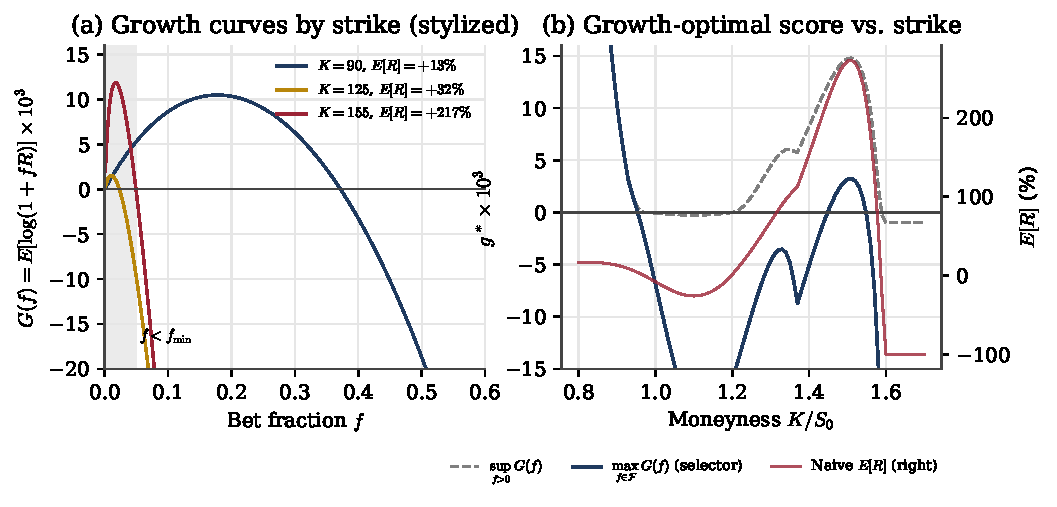
\includegraphics[width=\linewidth]{figures/fig4_kelly_illustration.pdf}
\caption{\emph{Stylized illustration, not estimated from data}: a 40-state law with a
diffuse body and a 4\% right-tail jump, calls priced at 30\% implied volatility, 120 DTE,
valued at intrinsic at the horizon. (a) Growth curves $G(f)$. The far-OTM strike ($K=155$)
has the largest $E[R]$ and a growth peak at $f\approx0.02$, inside the excluded region
$f<f_{\min}$. (b) Continuous-stake supremum growth (dashed), the selector's grid score
(solid) and naive $E[R]$ across strikes.}\label{fig:kelly}
\end{figure}

\paragraph{Validation: the selector finds the trade's direction on its own.} Nothing in the
selector specifies whether to buy calls or puts. Figure~\ref{fig:putshare} shows that it
still recovers the PEAD direction: puts are chosen for 32\% of D1 events and 5\% of D10
events, and the put share falls almost monotonically in between. Calls dominate
unconditionally because the law is centered on the positive trailing market drift. Across
picks the mean full-Kelly fraction is 13.8\%, and the Kelly pick differs from the naive-EV
pick on 29.8\% of events.

\begin{figure}[t]\centering
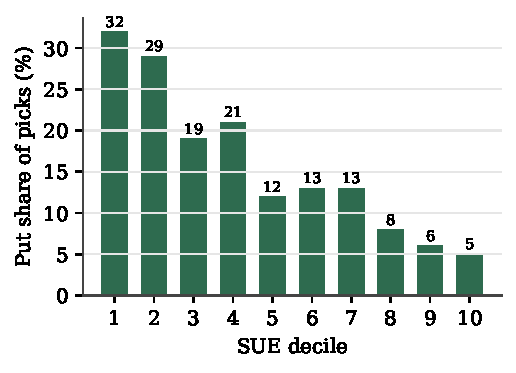
\includegraphics[width=0.55\linewidth]{figures/fig5_put_share.pdf}
\caption{Share of Kelly-optimal picks that are puts, by SUE decile; 113{,}927 walk-forward-scored events.}\label{fig:putshare}
\end{figure}

\subsection{From single-bet Kelly to a portfolio: the premium budget}

A typical quarter has about 1{,}200--1{,}300 positive-edge candidates. Their single-bet
fractions add up to around 170 NAVs, so staking each at $f^\ast$ is infeasible. Let $O_q$ be
the premium still outstanding from earlier cohorts. The quarter's new budget and allocation are
\begin{equation}
  B_q=\big(c\,V_q-O_q\big)^+,\qquad
  \pi_i=B_q\,\frac{h_i}{\sum_{j\in\mathcal{C}_q}h_j},\qquad h_i=\tfrac12 f^\ast_{k^\ast(i)},
  \label{eq:alloc}
\end{equation}
and each position buys $\lfloor \pi_i/(100\,P_i)\rfloor$ contracts. A 3\% round-trip cost on
premium is charged at entry. Positions are marked at quoted mids on days
$\{1,5,10,20,40,60\}$ and exit at day 60. The outstanding-premium test covers
\emph{overlapping} cohorts. An earlier implementation applied the budget to each entry
cohort alone, which let open premium exceed $c$ and produced an overstated 15.31\% return.
That result is kept only as a flagged historical comparison (Section~\ref{sec:audit}).

\begin{proposition}[Proportional allocation is fractional Kelly]\label{prop:fractional}
(a) The half-Kelly factor in \eqref{eq:alloc} cancels, so $\pi_i=\lambda_q f^\ast_i$ with
$\lambda_q=B_q/\sum_j f^\ast_j$. The book is Kelly-proportional in \emph{relative} sizing,
and its absolute scale is set entirely by the budget $c$.
(b) Assume independent bets and the quadratic approximation of
Proposition~\ref{prop:sharpe}. Scaling the vector of single-bet Kelly stakes by
$\lambda\in(0,1]$ gives portfolio growth $(2\lambda-\lambda^2)\sum_i g^\ast_i$ and a portfolio
Sharpe ratio
\begin{equation}
  \mathrm{SR}_{\text{port}}=\frac{\sum_i \mu_i^2/m_i}{\big(\sum_i \mu_i^2\sigma_i^2/m_i^2\big)^{1/2}},
\end{equation}
which does not depend on $\lambda$ and grows as $\sqrt{N}$ in the number of bets.
(c) Every position's loss is bounded by its premium. The loss on the positions open at any
moment is therefore at most $c$ times the NAV at which they were sized.
\end{proposition}

\noindent With $\sum_j f^\ast_j\approx 175$ and $c=0.3$, the book runs at
$\lambda\approx 1.7\times10^{-3}$ of full Kelly. It is a deeply fractional Kelly portfolio.
Its high Sharpe ratio comes from breadth, as part (b) predicts, not from leverage. The
empirical implied information coefficient is $3.49/\sqrt{4{,}770}\approx 0.05$. Part (b)
also predicts that return and volatility scale roughly linearly in $c$ while the Sharpe
ratio stays approximately unchanged. Table~\ref{tab:budget} confirms this: going from
$c=20\%$ to 30\% to 40\% moves return from 8.58\% to 12.26\% to 15.79\% and volatility
from 2.18\% to 3.33\% to 4.50\%, while Sharpe decays only mildly (3.78, 3.49, 3.28).
Compounding, whole-contract rounding and the overlap constraint account for the decay.

\begin{table}[t]\centering\small
\caption{Kelly options book: annualized return (Sharpe) by holding horizon and outstanding-premium budget $c$, with the near-ATM heuristic for comparison.}\label{tab:budget}
\footnotesize\setlength{\tabcolsep}{4pt}
\begin{tabular}{lrrrrrr}
\toprule
 & $+1$d & $+5$d & $+10$d & $+20$d & $+40$d & $+60$d\\
\midrule
$c=20\%$ & $-0.01\%$ ($-0.02$) & 1.96\% (1.77) & 3.49\% (1.95) & 5.74\% (2.49) & 8.08\% (2.96) & 8.58\% (3.78)\\
$c=30\%$ & $-0.18\%$ ($-0.26$) & 2.76\% (1.62) & 5.03\% (1.82) & 8.41\% (2.36) & 11.81\% (2.84) & \textbf{12.26\% (3.49)}\\
$c=40\%$ & $-0.36\%$ ($-0.39$) & 3.57\% (1.55) & 6.59\% (1.76) & 11.08\% (2.30) & 15.62\% (2.79) & 15.79\% (3.28)\\
Near-ATM & $-1.01\%$ ($-0.78$) & 0.78\% (0.31) & 2.13\% (0.60) & 2.91\% (0.60) & 4.67\% (0.72) & 9.51\% (1.04)\\
\midrule
Max DD, $+60$d & \multicolumn{6}{l}{$c=20\%$: $-10.3\%$;\ \ $c=30\%$: $-17.4\%$;\ \ $c=40\%$: $-23.9\%$;\ \ near-ATM: $-25.9\%$}\\
\bottomrule
\end{tabular}
\end{table}

Returns increase with horizon, which is exactly the decay profile of
Section~\ref{sec:decay}: a 3\% round-trip cost cannot be earned back from a one-day drift of
0.8\%, but it can be from 60 days of accumulated drift. Replacing the heuristic with the
Kelly selector at equal horizon triples the Sharpe ratio and cuts the drawdown by more than
half, largely because the heuristic funded only 2{,}007 of 99{,}294 signals, while the
proportional allocation spreads the budget over all of them.

%=====================================================================================
\section{Results}\label{sec:results}
%=====================================================================================

\begin{figure}[t]\centering
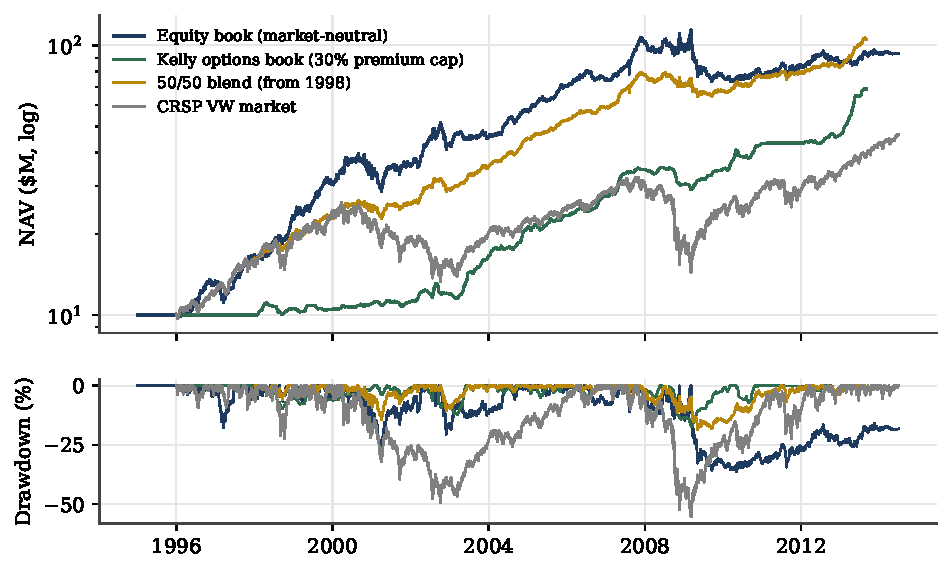
\includegraphics[width=\linewidth]{figures/fig6_nav_drawdown.pdf}
\caption{NAV (log scale, \$10M start) and drawdowns. The options book is flat through its
8-quarter walk-forward warm-up (1996--1997). The blend begins in 1998.}\label{fig:nav}
\end{figure}

\begin{table}[t]\centering\small
\caption{Risk profile of the two books. Summary statistics come from the committed backtest
summaries. Rows marked $\ddagger$ are computed from the daily NAV series over each book's
\emph{active} period (equity from 1996-01; options from 1998-01).}\label{tab:risk}
\begin{tabular}{lrr}
\toprule
 & Equity book & Options book ($c=30\%$, 60d)\\
\midrule
Annualized return (full window) & 12.15\% & 12.26\%\\
Annualized volatility & 12.20\% & 3.33\%\\
Sharpe ratio & 1.00 & 3.49\\
Maximum drawdown (trough date) & $-36.5\%$ (2010-05-07) & $-17.4\%$ (2009-03-11)\\
Final NAV from \$10M & \$93.3M & \$68.8M\\
\midrule
CAGR, active period$^\ddagger$ & 12.85\% & 14.06\%\\
Sharpe, active period$^\ddagger$ & 1.03 & 3.73\\
Sortino$^\ddagger$ & 1.39 & 5.88\\
Skewness / kurtosis of daily returns$^\ddagger$ & $-0.22$ / 10.1 & $+0.99$ / 11.0\\
Daily 99\% VaR / CVaR$^\ddagger$ & $-2.13\%$ / $-3.05\%$ & $-0.48\%$ / $-0.70\%$\\
Market beta / correlation$^\ddagger$ & $-0.015$ / $-0.02$ & $0.034$ / $0.20$\\
CAPM alpha, annualized ($t$-stat)$^\ddagger$ & 13.0\% (4.47) & 12.9\% (14.26)\\
Calmar ratio$^\ddagger$ & 0.35 & 0.81\\
\midrule
Positions & 119{,}130 (avg.\ 1{,}406 open) & 74{,}926 sized of 81{,}605 eligible\\
Realized gross / NAV$^\ddagger$ & avg.\ 4.5$\times$, max 7.6$\times$ & max open premium 29.3\% of NAV\\
Share of positions at ADV cap & 27.9\% & --\\
\bottomrule
\end{tabular}
\end{table}

\subsection{Standalone performance}

Table~\ref{tab:risk} and Figure~\ref{fig:nav} summarize the two books. They reach similar
returns through very different risk profiles. The equity book is a linear, market-hedged
long/short: negative skew, fat tails, a $-36.5\%$ drawdown, and no market beta. The options
book is convex and budget-constrained: positive skew, daily tail losses about four times
smaller, and a structural loss bound (Proposition~\ref{prop:fractional}c). It carries a
modest market correlation of $0.20$, which comes from its unconditional call bias. For
both books the CAPM alpha is essentially the whole return.

\subsection{Complementarity}

The two books are almost orthogonal: daily correlation $-0.055$ and monthly correlation
$-0.12$ over 175 months. Calendar-year returns (Table~\ref{tab:calendar}, Figure~\ref{fig:cal})
show why. In 2009 the equity book lost 23.2\%, its worst year, while the options book gained
14.3\%. The 2009 rebound was a rally in low-quality, heavily shorted names, the same regime
that produces momentum crashes \citep{DanielMoskowitz2016}. A linear short book pays for
such a rally without limit. A long put pays at most its premium, and long calls on
positive-surprise names take part in the rally.

\begin{table}[t]\centering\small
\caption{Calendar-year returns (\%). The options book has no data for 2011: that year's
OptionMetrics price file is corrupt in the source extract. Its 2012 figure includes
positions whose holding windows straddled the gap, and its 2013 figure covers January to
August only.}\label{tab:calendar}
\begin{tabular}{lrrr@{\hspace{2em}}lrrr}
\toprule
Year & Equity & Options & Market & Year & Equity & Options & Market\\
\midrule
1996 & 33.1 & -- (warm-up) & 21.3 & 2005 & 23.0 & 9.7 & 7.3\\
1997 & 26.1 & -- (warm-up) & 30.4 & 2006 & 5.0 & 17.8 & 16.2\\
1998 & 37.1 & 5.4 & 22.3 & 2007 & 37.3 & 25.9 & 7.4\\
1999 & 35.9 & $-0.5$ & 25.7 & 2008 & $-1.6$ & $-12.0$ & $-38.2$\\
2000 & 12.6 & 4.9 & $-11.3$ & 2009 & $-23.2$ & 14.3 & 31.2\\
2001 & 2.8 & 2.2 & $-11.0$ & 2010 & $-0.1$ & 24.5 & 17.7\\
2002 & 18.7 & 6.4 & $-20.9$ & 2011 & 9.6 & n/a & $-1.1$\\
2003 & 6.1 & 38.5 & 33.2 & 2012 & 2.2 & 7.1 & 15.8\\
2004 & 25.9 & 28.5 & 13.0 & 2013 & 7.4 & 48.3 (Jan--Aug) & 30.5\\
\bottomrule
\end{tabular}
\end{table}

\begin{figure}[t]\centering
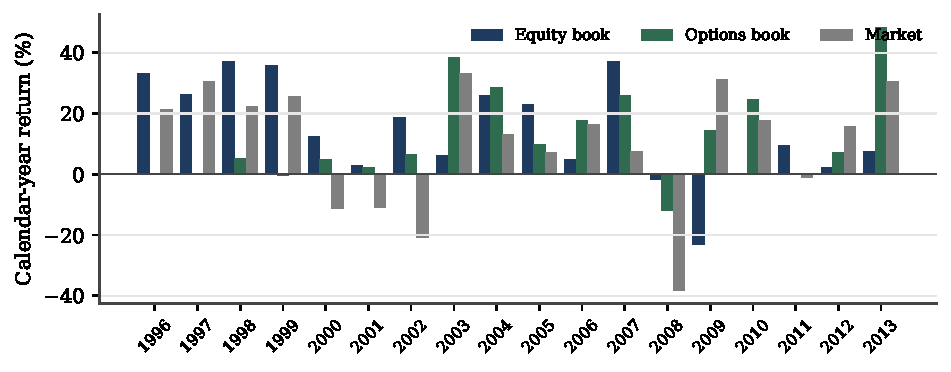
\includegraphics[width=\linewidth]{figures/fig7_calendar_returns.pdf}
\caption{Calendar-year returns of both books against the CRSP value-weighted market.}\label{fig:cal}
\end{figure}

Table~\ref{tab:blend} reports static blends, rebalanced daily with zero rebalancing cost,
over the options book's active window. At 50/50 the blend keeps the return of either
book (12.7\%), roughly doubles the equity book's Sharpe ratio (0.94 to 1.88 in this window)
and halves its drawdown. The in-sample tangency portfolio puts about 92\% on the options
book. We do not recommend that allocation: the options book's capacity and cost
assumptions (Section~\ref{sec:limits}) are much less certain than its Sharpe ratio
suggests, and the equity book diversifies model risk as well as market risk.

\begin{table}[h]\centering\small
\caption{Static blends, 1998-01-06 to 2013-08-30 (3{,}939 days; options returns set to zero on dates absent from its calendar).}\label{tab:blend}
\begin{tabular}{rrrrr}
\toprule
Equity weight & CAGR & Vol & Sharpe & Max DD\\
\midrule
100\% & 11.82\% & 12.68\% & 0.94 & $-36.5\%$\\
75\% & 12.33\% & 9.50\% & 1.27 & $-25.6\%$\\
50\% & 12.73\% & 6.48\% & 1.88 & $-18.5\%$\\
25\% & 12.99\% & 3.98\% & 3.09 & $-15.0\%$\\
0\% & 13.13\% & 3.44\% & 3.61 & $-17.4\%$\\
\bottomrule
\end{tabular}
\end{table}

\subsection{Capacity and risk-budget frontiers}

\begin{figure}[t]\centering
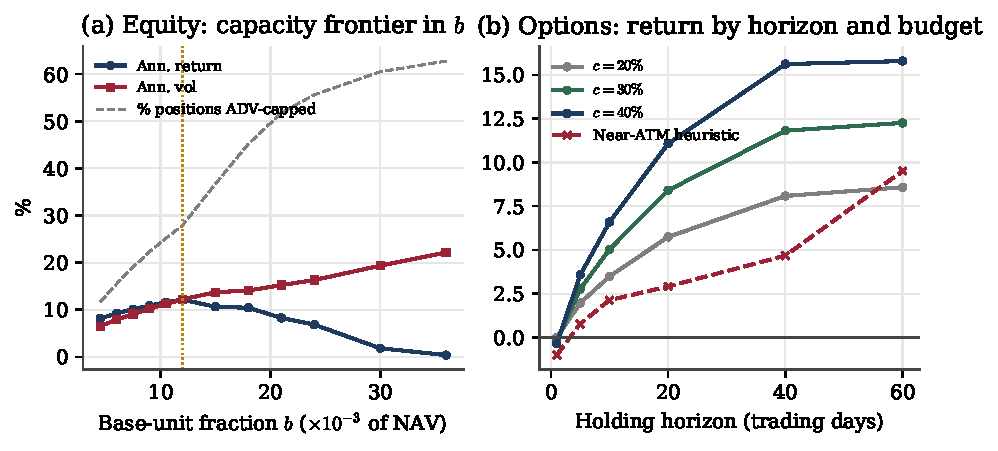
\includegraphics[width=\linewidth]{figures/fig8_frontiers.pdf}
\caption{(a) Equity: return, volatility and the share of ADV-capped positions against the
base-unit fraction $b$. The dotted line marks the chosen $b=0.012$. (b) Options: annualized
return against holding horizon for three premium budgets and for the near-ATM
heuristic.}\label{fig:frontiers}
\end{figure}

Figure~\ref{fig:frontiers} shows the main difference between the two books as scalable
products. Equity return is capacity-bound: the frontier bends over at a finite $b$
(Proposition~\ref{prop:capacity}). Options return is budget-bound: to first order it
scales linearly with $c$, and $c$ is a risk-appetite dial with a hard loss interpretation.
The practical limits on the options book lie outside the backtest: quoted width, depth
and market impact in single-name options.

%=====================================================================================
\section{Statistical robustness and backtest hygiene}\label{sec:audit}
%=====================================================================================

\subsection{Multiple testing}

Both books were selected from a family of trials, so we deflate their Sharpe ratios
\citep{BaileyLopezdePrado2014}. For $N$ trials whose annualized Sharpe ratios have
variance $V$, the expected maximum under the null is
\begin{equation}
  \widehat{\mathrm{SR}}_0=\sqrt{V}\Big[(1-\gamma_E)\,\Phi^{-1}\!\big(1-\tfrac1N\big)+\gamma_E\,\Phi^{-1}\!\big(1-\tfrac{1}{Ne}\big)\Big],
\end{equation}
where $\gamma_E$ is the Euler--Mascheroni constant. The deflated Sharpe ratio is the
probabilistic Sharpe ratio \citep{BaileyLopezdePrado2012} measured against
$\widehat{\mathrm{SR}}_0$, allowing for the skewness and kurtosis of the returns:
\begin{equation}
  \mathrm{DSR}=\Phi\!\left(\frac{(\widehat{\mathrm{SR}}-\widehat{\mathrm{SR}}_0)\sqrt{T-1}}{\sqrt{1-\hat\gamma_3\widehat{\mathrm{SR}}+\tfrac{\hat\gamma_4-1}{4}\widehat{\mathrm{SR}}^2}}\right),
\end{equation}
with Sharpe ratios in per-period units. The results are:
\begin{itemize}
  \item \textbf{Equity:} $N=93$ (every point of the aggressive sizing sweep across all
        designs), $\widehat{\mathrm{SR}}_0=0.66$, $\mathrm{DSR}=0.94$. The book beats the
        best-of-93 null with 94\% probability, just short of the conventional 95\%. A
        committee should read the equity book's Sharpe ratio as \emph{probably but not
        conclusively} greater than what selection alone would produce. The signal behind it
        is unambiguous ($t$-statistics of 5 to 14 in Section~\ref{sec:evidence}); the
        uncertainty is about how well the portfolio's calibration generalizes.
  \item \textbf{Options:} $N=24$ (four constructions $\times$ six horizons),
        $\widehat{\mathrm{SR}}_0=2.56$, $\mathrm{DSR}>0.9999$.
\end{itemize}
These trial counts are lower bounds. Earlier exploratory sweeps (trim, tilt, leverage cap)
widen the family. Even doubling $N$ moves $\widehat{\mathrm{SR}}_0$ only by roughly the
change in $\Phi^{-1}(1-1/N)$, from about 2.3 to 2.6 standard deviations.

\subsection{Audit log: defects found and corrected}

Table~\ref{tab:audit} lists every defect the development process caught. We report them
because the \emph{direction} of each correction shows how fragile each headline number
is. Every correction lowered or left unchanged the reported performance.

\begin{table}[t]\centering\small
\caption{Backtest defects detected and corrected during development.}\label{tab:audit}
\begin{tabularx}{\linewidth}{@{}p{3.2cm}Xp{3.3cm}@{}}
\toprule
Defect & Symptom that exposed it & Effect of the fix\\
\midrule
Sharpe denominator & Daily returns divided by initial rather than prior-day NAV, overstating volatility as NAV compounded & Sharpe ratios rose; returns and drawdowns unchanged\\
EAR leakage & Day-0-to-day-1 return overlapped the first day of held P\&L; Sharpe rose monotonically with EAR weight & Sharpe flat at 1.00--1.06; EAR not adopted\\
Ambient beta in return law & Selector chose calls even in D1 (1996--2013 was a net up market) & Shape from market-adjusted returns, re-centered on trailing drift\\
OptionMetrics strike units & Strikes stored $\times1000$; puts dominated even D10 with Kelly fractions near 1 (a ``free money'' artifact) & Strikes divided by 1000 at source\\
Full-sample return law & 1998 trades priced with 2013 data & Walk-forward law, 8-quarter warm-up; Sharpe about 4.0 $\to$ 3.56\\
Independent Kelly sizing & Budget exhausted by a few bets; 46 positions funded in 17 years & Kelly-proportional allocation of a shared budget\\
Per-cohort premium cap & Open premium could exceed $c$ across overlapping 60-day cohorts & Cap on total outstanding premium; 15.31\% $\to$ 12.26\% (at $c=30\%$)\\
Data drift on a staged copy & 40\% of decay-day cells changed with no code change & Results restored to canonical data; checksum manifest and pre-commit hook\\
\bottomrule
\end{tabularx}
\end{table}

We also inspected the day-level P\&L of the options book. Its worst days fall on
2008-10-24, 2008-11-20 and September 2002, which are real stress episodes, not artifacts of
a smoothed P\&L.

%=====================================================================================
\section{Limitations and implementation risk}\label{sec:limits}
%=====================================================================================

We list these without softening. Each item is either a reason realized performance would be
lower or a test still to be run.

\begin{enumerate}
\item \textbf{Sample period.} All results are for 1996--2013, and the era analysis shows a
      weakening drift after 2008. A data extension through the present and a
      post-publication decay adjustment \citep{McLeanPontiff2016} are required before any
      capital is allocated.
\item \textbf{Intra-quarter ranking.} Deciles are formed from each announcement quarter's
      full cross-section, so an early-quarter event is ranked partly against announcements
      that come later. This is a mild look-ahead that the literature commonly accepts. A
      tradeable version must rank against trailing breakpoints, for example the previous
      quarter's SUE distribution.
\item \textbf{In-sample calibration of the equity book.} The decay-day holding periods, the
      trim and tilt, and the base-unit fraction were all chosen on the full sample. The DSR
      of 0.94 reflects this; a walk-forward re-estimation of $H_c$ and $b$ is the obvious
      next test. (A walk-forward ML extension, ``Strategy~8'', exists but ran on an
      unverified data copy and is excluded here.)
\item \textbf{Equity costs and leverage.} Costs are 5--25 bp per side by liquidity
      quintile. Borrow fees, index-hedge costs and financing are not modeled. At the chosen
      sizing, 27.9\% of positions sit at 5\% of ADV, where impact is likely to exceed the
      modeled cost \citep{FrazziniIsraelMoskowitz2018,NovyMarxVelikov2016}. The gross cap
      $L=6$ applies per entry cohort. Across overlapping cohorts, realized gross averages
      4.5$\times$ NAV and peaks at 7.6$\times$, which is prime-brokerage-level leverage.
\item \textbf{Option execution.} Entries and marks use mids with a flat 3\% round-trip
      charge. Quoted single-name spreads, especially on OTM strikes and in the early
      sample, are often wider. Missing forward quotes are forward-filled. The book opens
      about 4{,}800 small positions a year; capacity and impact
      have not been modeled. Replacing the flat charge with the actual quoted bid/ask on
      the selected contracts is the single most important robustness test outstanding.
\item \textbf{Options data coverage.} 2011 is missing because its source file is corrupt,
      so the trading-day calendar compresses across the gap, and 2013 ends in August. The
      matched sample is tilted toward names with liquid, longer-dated chains.
\item \textbf{Return-law pooling.} One distribution per (decile, quarter) is shared by every
      stock in the decile, regardless of its own volatility. Scaling the states by each
      stock's volatility (or implied volatility) should sharpen strike selection and is not
      yet built.
\item \textbf{Universe.} Only stocks with listed options at some point in the window are
      included. Micro-caps with no options, where PEAD is historically strongest, are
      excluded. That makes the equity results conservative in magnitude but relevant to a
      liquid mandate.
\end{enumerate}

%=====================================================================================
\section{Conclusion}
%=====================================================================================

PEAD in this sample passes the tests an allocator should require. It is significant under
earnings-season clustering. It survives, and grows under, a size/value characteristic
benchmark. It is homogeneous across industries, graded by size as limits to arbitrage
predicts, and confirmed in a second, independently priced market. We harvest it in two
ways that are complementary in both mathematics and risk. The linear book neutralizes every
unpriced exposure we could measure and scales to its capacity optimum, which yields about
12\% a year with no market beta. The convex book treats each event as a bet on an
empirical distribution, picks the strike that maximizes expected log growth, and sizes the
book as a deeply fractional Kelly portfolio under a hard premium budget, which also yields
about 12\% a year, with a Sharpe ratio driven by breadth and losses bounded by
construction. The two books are close to orthogonal and hedge each other's worst regime,
so they are best considered together. The work that remains before deployment is concrete:
data after 2013, trailing-breakpoint ranking, walk-forward calibration of the equity book,
and quote-level option execution costs.

\vspace{1em}
\noindent\fbox{\parbox{\dimexpr\linewidth-2\fboxsep-2\fboxrule}{\footnotesize
\textbf{Important disclosure.} All performance figures in this paper are hypothetical and
come from historical backtests. They do not reflect actual trading, and they benefit from
hindsight in model design. Backtested results have inherent limitations, including the
modeling assumptions in Section~\ref{sec:limits}; realized results may differ materially.
Nothing here is an offer, a solicitation, or investment advice.}}

%=====================================================================================
\appendix
\section{Proofs}\label{app:proofs}
%=====================================================================================

\paragraph{Proof of Proposition~\ref{prop:neutral}.}
Fix $q$ and side $\sigma$. For an occupied group $g$,
$\sum_{i\in g}|\tilde w_i|=\sum_{i\in g}|t_i|\big/\big(\sum_{j\in g}|t_j|\cdot N_{q\sigma}\big)=1/N_{q\sigma}$,
which proves (b). Summing over the $N_{q\sigma}$ groups of the side gives
$\sum_{i\in q\sigma}|\tilde w_i|=1$ for both sides. Every weight on a side has the same sign,
so $\sum_{w>0}\tilde w=1=-\sum_{w<0}\tilde w$. The global rescaling in \eqref{eq:weights}
multiplies every weight by the same positive constant, which proves (a). For (c), sector
$k$'s long gross is the sum over its occupied long groups, $n^+_k/N_{q+}$, and likewise on
the short side. Net exposure is the difference, and it vanishes when
$n^{+}_{k}/N_{q+}=n^{-}_{k}/N_{q-}$, in particular when both sides occupy the same set of
cells. The size argument is symmetric. $\square$

\paragraph{Proof of Proposition~\ref{prop:capacity}.}
Fix a cohort. By \eqref{eq:notional}, $\partial n_i/\partial b=|w_i|V_q\,\1\{|w_i|bV_q<\kappa\mathrm{ADV}_i\}$.
Position $i$ stops absorbing marginal capital at $b_i=\kappa\mathrm{ADV}_i/(|w_i|V_q)$, and
this threshold increases in $\mathrm{ADV}_i$. Write
$\mathcal{U}(b)=\{i: b<b_i\}$ for the uncapped set, which shrinks as $b$ grows. The marginal
alpha per marginal gross dollar is the $|w|$-weighted average of $\alpha_i$ over
$\mathcal{U}(b)$. Raising $b$ removes the members with the smallest $b_i$, which by the
monotonicity of $b_i$ in ADV are the smallest names, and hence, under the assumption, those
with the largest $\alpha_i$. The weighted average therefore cannot increase. Expected
arithmetic P\&L, the integral of this non-increasing marginal alpha, is concave in $b$.
Volatility is non-decreasing in gross, so
$\mu(b)-\tfrac12\sigma^2(b)$ is concave with $\mu(0)=\sigma(0)=0$. Its derivative at zero is
positive when the uncapped book has positive alpha. As $b\to\infty$, alpha saturates while
the variance term does not, so the function eventually decreases, and the maximum is
interior. $\square$

\paragraph{Proof of Proposition~\ref{prop:wellposed}.}
$R_{k,s}\ge-1$ and $f\le0.95$ give $1+fR_{k,s}\ge0.05$. The second derivative is
$G''_k(f)=-\sum_sp_sR_{k,s}^2/(1+fR_{k,s})^2<0$ unless every $R_{k,s}=0$. Direct evaluation
gives $G_k(0)=0$ and $G_k'(0)=\sum_sp_sR_{k,s}$. Since $G_k$ is concave, its continuum
maximizer on $[0,1)$ is positive if and only if $G_k'(0)>0$. $\square$

\paragraph{Proof of Proposition~\ref{prop:sharpe}.}
Substitute the expansion of the logarithm and take expectations, which gives
$G_k(f)=f\mu_k-\tfrac12f^2m_k+O(f^3\E|R_k|^3)$. Maximizing the quadratic gives
$f^\ast=\mu_k/m_k$ and $g^\ast=\mu_k^2/(2m_k)$. Dividing numerator and denominator by
$\sigma_k^2$ gives $\tfrac12\mathrm{SR}_k^2/(1+\mathrm{SR}_k^2)$, which is increasing in
$\mathrm{SR}_k$ for $\mathrm{SR}_k>0$. $\square$

\paragraph{Proof of Proposition~\ref{prop:hurdle}.}
The selected contract maximizes $g^\ast_k=\max_{f\in\F}G_k(f)$ and is traded only if that
maximum is positive. $G_k$ is concave with $G_k(0)=0$. If $G_k(f_{\min})\le0$, then
concavity gives $G_k(f)\le (f/f_{\min})\,G_k(f_{\min})$ for every $f\ge f_{\min}$, so
$G_k(f)\le 0$ on all of $\F$. Selectability therefore requires $G_k(f_{\min})>0$. In the
quadratic approximation this is $f_{\min}\mu_k-\tfrac12f_{\min}^2m_k>0$, which is
\eqref{eq:hurdle}. $\square$

\paragraph{Proof of Proposition~\ref{prop:fractional}.}
(a) $h_i/\sum_jh_j=f^\ast_i/\sum_jf^\ast_j$. (b) Under independence and the quadratic
approximation, portfolio growth is $\sum_i(\pi_i\mu_i-\tfrac12\pi_i^2m_i)$. Setting
$\pi_i=\lambda\mu_i/m_i$ gives
\[
\sum_i\frac{\mu_i^2}{m_i}\Big(\lambda-\tfrac12\lambda^2\Big)=(2\lambda-\lambda^2)\sum_ig^\ast_i .
\]
The
portfolio mean is $\lambda\sum_i\mu_i^2/m_i$ and its standard deviation is
$\lambda(\sum_i\mu_i^2\sigma_i^2/m_i^2)^{1/2}$, so $\lambda$ cancels in their ratio. With $N$
bets of comparable size the numerator is $O(N)$ and the denominator $O(\sqrt N)$.
(c) A long option position costs its premium and has a non-negative payoff, so its loss is
at most the premium. Premium outstanding is at most $cV_q$ by construction of $B_q$. $\square$

%=====================================================================================
\section{Parameter summary and reproducibility map}
%=====================================================================================

\begin{table}[h]\centering\small
\begin{tabularx}{\linewidth}{@{}lX@{}}
\toprule
\multicolumn{2}{@{}l}{\textbf{Equity book}}\\
Signal & Within-quarter percentile of analyst SUE; trim $\tau=0.15$, tilt $\gamma=1$\\
Neutrality & Dollar-neutral per cohort; equal gross per (FF12 sector $\times$ size quintile) group per side\\
Holding period & Cell decay day $H_c$ (Section~\ref{sec:decay}); 31--200 trading days\\
Sizing & $b=0.012$ of trailing NAV per unit weight; ADV cap 5\% of 21-day dollar volume; cohort gross cap $6\times$ NAV with priority trimming\\
Costs & 25/15/10/7/5 bp per side by liquidity quintile\\
\midrule
\multicolumn{2}{@{}l}{\textbf{Options book}}\\
Universe & All strikes, single expiry closest to 120 DTE ($\ge95$), up to 60 contracts per event\\
Return law & Walk-forward, decile-conditioned, 40 equal-mass quantile states, 60-day horizon, 8-quarter warm-up\\
Selection & $\arg\max_k\max_{f\in\{0.05,\dots,0.95\}}\E[\log(1+fR_k)]$; trade iff $g^\ast>0$\\
Sizing & Outstanding-premium budget $c=30\%$ of trailing NAV, allocated in proportion to $f^\ast$\\
Holding / costs & 60 trading days, marked at quoted mids; 3\% round-trip on premium\\
\bottomrule
\end{tabularx}
\end{table}

\noindent\textbf{Code.} Evidence: \texttt{scripts/equity\_pead/01--10};
options evidence: \texttt{scripts/options\_pead/33--39}; equity book:
\texttt{scripts/equity\_strategy/14--16} (decay and positions), \texttt{24} (construction),
\texttt{36} (sizing frontier); options book: \texttt{scripts/options\_strategy/46}
(return law), \texttt{47/47b} (chains), \texttt{48} (selector), \texttt{49--50} (pricing and
backtest). The supplementary statistics in this paper (risk moments, DSR, blends, calendar
returns) and all figures come from \texttt{scripts/build\_quant\_paper\_figures.py}, which
writes \texttt{reports/paper/paper\_stats.json}.

%=====================================================================================
\begin{thebibliography}{99}\small
%=====================================================================================
\bibitem[Bailey and L\'opez de Prado(2012)]{BaileyLopezdePrado2012}
Bailey, D.~H., and M.~L\'opez de Prado (2012). The Sharpe ratio efficient frontier.
\textit{Journal of Risk} 15(2), 3--44.

\bibitem[Bailey and L\'opez de Prado(2014)]{BaileyLopezdePrado2014}
Bailey, D.~H., and M.~L\'opez de Prado (2014). The deflated Sharpe ratio: correcting for
selection bias, backtest overfitting, and non-normality. \textit{Journal of Portfolio
Management} 40(5), 94--107.

\bibitem[Ball and Brown(1968)]{BallBrown1968}
Ball, R., and P.~Brown (1968). An empirical evaluation of accounting income numbers.
\textit{Journal of Accounting Research} 6(2), 159--178.

\bibitem[Bernard and Thomas(1989)]{BernardThomas1989}
Bernard, V.~L., and J.~K.~Thomas (1989). Post-earnings-announcement drift: delayed price
response or risk premium? \textit{Journal of Accounting Research} 27 (Supplement), 1--36.

\bibitem[Bernard and Thomas(1990)]{BernardThomas1990}
Bernard, V.~L., and J.~K.~Thomas (1990). Evidence that stock prices do not fully reflect
the implications of current earnings for future earnings. \textit{Journal of Accounting and
Economics} 13(4), 305--340.

\bibitem[Daniel et~al.(1997)]{DGTW1997}
Daniel, K., M.~Grinblatt, S.~Titman, and R.~Wermers (1997). Measuring mutual fund
performance with characteristic-based benchmarks. \textit{Journal of Finance} 52(3),
1035--1058.

\bibitem[Daniel and Moskowitz(2016)]{DanielMoskowitz2016}
Daniel, K., and T.~J.~Moskowitz (2016). Momentum crashes. \textit{Journal of Financial
Economics} 122(2), 221--247.

\bibitem[DellaVigna and Pollet(2009)]{DellaVignaPollet2009}
DellaVigna, S., and J.~M.~Pollet (2009). Investor inattention and Friday earnings
announcements. \textit{Journal of Finance} 64(2), 709--749.

\bibitem[Fama and MacBeth(1973)]{FamaMacBeth1973}
Fama, E.~F., and J.~D.~MacBeth (1973). Risk, return, and equilibrium: empirical tests.
\textit{Journal of Political Economy} 81(3), 607--636.

\bibitem[Frazzini et~al.(2018)]{FrazziniIsraelMoskowitz2018}
Frazzini, A., R.~Israel, and T.~J.~Moskowitz (2018). Trading costs. Working paper, AQR
Capital Management.

\bibitem[Grinold(1989)]{Grinold1989}
Grinold, R.~C. (1989). The fundamental law of active management. \textit{Journal of
Portfolio Management} 15(3), 30--37.

\bibitem[Hirshleifer et~al.(2009)]{HirshleiferLimTeoh2009}
Hirshleifer, D., S.~S.~Lim, and S.~H.~Teoh (2009). Driven to distraction: extraneous events
and underreaction to earnings news. \textit{Journal of Finance} 64(5), 2289--2325.

\bibitem[Kelly(1956)]{Kelly1956}
Kelly, J.~L. (1956). A new interpretation of information rate. \textit{Bell System
Technical Journal} 35(4), 917--926.

\bibitem[MacLean et~al.(2011)]{MacLeanThorpZiemba2011}
MacLean, L.~C., E.~O.~Thorp, and W.~T.~Ziemba, eds. (2011). \textit{The Kelly Capital Growth
Investment Criterion: Theory and Practice}. World Scientific.

\bibitem[McLean and Pontiff(2016)]{McLeanPontiff2016}
McLean, R.~D., and J.~Pontiff (2016). Does academic research destroy stock return
predictability? \textit{Journal of Finance} 71(1), 5--32.

\bibitem[Mendenhall(2004)]{Mendenhall2004}
Mendenhall, R.~R. (2004). Arbitrage risk and post-earnings-announcement drift.
\textit{Journal of Business} 77(4), 875--894.

\bibitem[Novy-Marx and Velikov(2016)]{NovyMarxVelikov2016}
Novy-Marx, R., and M.~Velikov (2016). A taxonomy of anomalies and their trading costs.
\textit{Review of Financial Studies} 29(1), 104--147.

\bibitem[Shleifer and Vishny(1997)]{ShleiferVishny1997}
Shleifer, A., and R.~W.~Vishny (1997). The limits of arbitrage. \textit{Journal of
Finance} 52(1), 35--55.
\end{thebibliography}

\end{document}
